\section{Interface Homme Machine}
	Dans toute application où les interactions avec l'utilisateur sont fréquentes, et notamment dans un jeu tel que la bataille navale, il est bon que cette application possède une interface homme machine(IHM) qui va prendre en compte les actions de l'utilisateur et modifier ce qu'il voit en conséquence. \newline
	
	Nous avons donc développé une IHM permettant à un joueur de pouvoir jouer aisément et sans difficultés qui va se découper en deux fenêtres principales. La première est la fenêtre de démarrage où l'utilisateur pourra définir les différentes options liées à la nouvelle partie et la seconde est l'interface principale du jeu où toute la partie se déroulera. Nous allons donc exposer ces deux fenêtres dans deux parties distinctes où nous expliquerons comment les fenêtres sont construites et détaillerons les différents actions a effectué. Enfin, nous en profiterons pour mettre en avant, dans une troisième partie, les composants graphiques permettant l'affichage des Boards. 
	
\subsection{La fenêtre de démarrage}
	Comme dit plus haut, la fenêtre de démarrage est la première fenêtre que verra le joueur au lancement de l'application. Pour nous aider à décrire cette fenêtre, voici une capture d'écran:
	
	\begin{figure}[!h]
		\centering
		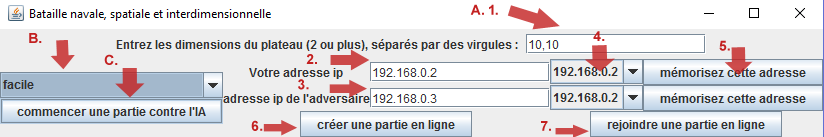
\includegraphics [width=10cm]{images/start_window.png}
		\caption{Fenêtre de démarrage de l'application}
		\label {startwindow}
	\end{figure}
	
	Comme on peut le voir, la fenêtre de démarrage est séparée en plusieurs morceaux. Pour s'y repérer, nous allons d'abord nous intéresser aux différents champs à remplir et actions à effectuer pour pouvoir créer une partie locale contre une IA, puis nous réitérerons cette logique pour pour soit créer, soit rejoindre une partie en ligne.
	
	\subsubsubsection{Une partie en local}
		Pour effectuer une partie en local, il faut premièrement indiquer, dans le champ de texte en haut à droite symbolisé par un "A", les dimensions de notre plateau de jeu, chaque dimension étant séparée par le symbole ",". Puis, nous devons choisir, grâce à la liste déroulante symbolisé par un "B" à gauche, le niveau de difficulté choisi pour l'IA qui sont, à l'heure actuelle, au nombres de trois. Enfin, Nous pouvons lancer la partie en cliquant sur le bouton "commencer une partie contre l'IA, qui se situe en bas à gauche symbolisé par un "C".

	\subsubsubsection{Une partie en réseau}
		Pour pouvoir jouer ligne, il faut, bien entendu, indiquer les dimensions du plateau de jeu, cependant cette information n'est nécessaire que pour le joueur qui hébergera la partie. Comme pour la partie en local, il faut remplir le champ de texte marqué d'un "1" en haut à droite de la fenêtre. Ensuite, chaque joueur doit rentrer son adresse IPv4 dans le champ numéroté "2" et l'adresse IPv4 de l'adversaire dans le champ numéro "3" au centre de la fenêtre. \newline
Il est également possible de récupérer une adresse mémorisé au préalable dans un fichier texte, apparaissant dans les liste déroulantes notés "4" mais aussi de mémoriser l'adresse, qui est écrite dans les champ de textes sus-mentionné, grâce aux boutons sur la droite.
\newline
Enfin, le joueur hôte lance la partie en cliquant sue le bouton "créer une partie en ligne", noté "6" en bas au centre de la fenêtre et le joueur invité peut rejoindre une partie après avoir cliqué sur le bouton indiqué par un "7".

\subsection{L'interface du jeu}
	\subsubsection{Le placement des bateaux}
		Avant de pouvoir jouer, il est nécessaire que les joueurs puissent placer leurs bateaux. Ce placement est illustré dans la figure suivante: \newline
		\begin{figure}[!h]
			\centering
			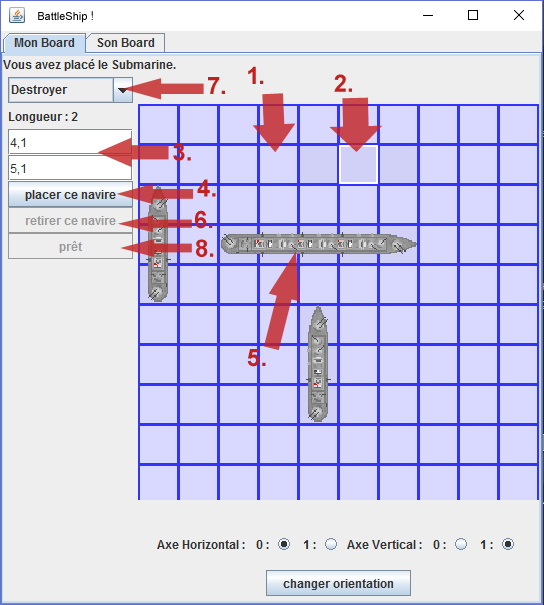
\includegraphics [width=5cm]{images/ship_placement.png}
			\caption{Placement des bateaux}
		\end{figure}
	
	Le  joueur doit avant tout cliquer sur une des cases du plateau de jeu, ce composant graphique un peu spécial sera explicité dans une autre sous-partie. La case cliquée représentera alors la proue du bateau("1") et, en cliquant sur une seconde case, nous choisissons la poupe("2") de celui-ci. Il est à noter que, sur la gauche de la fenêtre, il est possible d'entrer les coordonnées des deux cases en format textuelle, c'est à dire "X,X"("3").
	\newline
	
	Il faut ensuite cliquer sur le bouton "Placer ce navire"("4"), en dessous des champs de texte permettant de renseigner les coordonnées. Le fait de cliquer sur ce bouton a pour effet de faire passer le bateau a placé au suivant dans la liste déroulante en haut à gauche("7"). Naturellement, il est aussi possible de retirer un navire précédemment placé en le choisissant dans cette même liste et en cliquant dur le bouton "retirer ce navire" ("6").
	\newline
	
	Enfin, une fois tous les bateaux placés, le bouton "prêt"("8") est activé et nous pouvons cliquer dessus pour débuter une partie.
	\newline
	
	Toutes ces étapes même au commencement de la partie. Nous allons donc maintenant décrire ce que l'utilisateur voit et peut faire lors d'un tour de jeu sur une partie déjà avancée.
	
	\subsubsection{Une partie typique}
	Pour comprendre l'interface mise en œuvre ici, il est nécessaire de pouvoir la visualiser correctement. Pour cela, une capture de la fenêtre est donnée ci-après:\newline
	\begin{figure}[!ht]
		\centering
		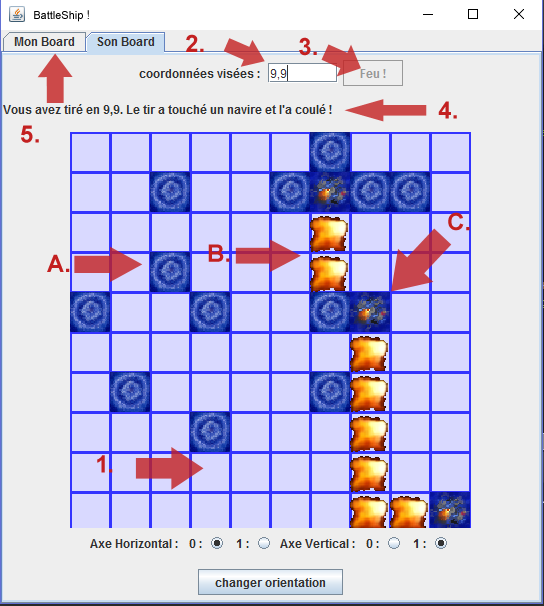
\includegraphics [width=5cm]{images/game_in_action.png}
		\caption{Une partie à un stade avancée}
	\end{figure}
	
	Sur cette image, nous pouvons tout d'abord parler du plateau de jeu. En effet, celui ci voit ses cases changées au cours de la partie suivant si la case a été ciblé on non ("1"). Si elle a été ciblé, cette case peut marqué comme "manqué" ("A"), "touchée" ("B") ou ecnore "coulée" ("C").
	\newline
	
	Lors du tour du joueur, celui-ci doit renseigner la case ou les coordonnées sur lesquelles il souhaite tirer. Il a donc à sa disposition la possibilité de soit cliquer directement sur la case voulue("1") ou alors de rentrer les coordonnées de la case au format textuel comme défini plus haut ("2"). Le joueur fait ensuite feu grâce au bouton "Feu!" ("3") et obtient le résultat de son tir qui affiche donc une image différente pour les trois cas possibles("A", "B" ou "C") ainsi qu'un petit texte décrivant la nature du résultat ("4"). Le joueur a également la possibilité de regarder son plateau de jeu, en cliquant sur l'onglet "Mon Board" ("5").
\newline

	Voici typiquement comment l'IHM s'arrange et les différentes actions que le joueur peut effectuer au cous d'une partie. 
	 \newline
	  
	Nous allons maintenant évoqué et expliqué le composant graphique majeur de l'application, le plateau de jeu qui se décline en plusieurs composants suivant quel plateau nous souhaitons regarder: soit le notre avec la position de nos bateaux, soit celui de l'adversaire contenant tous les résultats de nos tirs.

\subsection{La représentation du plateau de jeu}
	La représentation d'un espace à deux, trois ou plus de dimensions se complexifie avec le nombre de dimensions.
Nous avons choisi de représenter les plateaux à deux dimensions de manière classique, une surface avec un quadrillage. La représentation des plateaux à trois dimensions utilise une succession de plateaux à deux dimensions empilés entre lesquels on peut naviguer facilement. \newline

	Pour les nombres de dimensions supérieures, nous avons fait le choix de ne pas tout représenter étant donné la difficulté de visualiser un espace à quatre dimensions pour les humains et l'absence de conventions communément partagées sur la représentation de cet espace.

\subsubsection{Explications sur les axes}

	Plutôt que de montrer une représentation qui ne serait pas comprise par les joueurs, nous avons opté pour un système de composantes fixes pour les dimensions non représentées. Ainsi, pour représenter un Board de dimensions (5, 5, 5, 5), on peut fixer la quatrième composante de chaque case représentée à la valeur t : les cases représentées seront celles dont les coordonnées sont (x, y, z, t) pour x, y et z entre 0 et 4, et pour t fixé. Les cases de coordonnées dont la quatrième composante n'est pas égale à t ne sont pas représentées.
\newline

	Nos composants graphiques utilisent des objets Coordinates d'une façon spéciale pour déterminer les axes et les coordonnées fixées.
	\newline	
	
	Dans ces coordonnées, les composantes de valeurs positives ou nulles représentent des composantes fixées et les valeurs -1, -2, -3 désignent respectivement qu'il faut représenter les composantes correspondantes sur l'axe X (horizontal, de gauche à droite), l'axe Y (vertical, de haut en bas) ou sur l'axe Z (en profondeur, vers l'écran).
\newline
	
	Exemple : Dans une représentation en 3 dimensions d'un Board de dimensions (5, 4, 5, 3, 6), si on fixe l'axe à (-1, 2, -3, 1, -2). Les cases représentées seront celles de coordonnées (a, 2, b, 1, c) avec a, b et c des valeurs entières dans les limites des dimensions du Board.
Chaque case sera représenté sera située à la a-ième place sur l'axe des X, la c-ième place sur l'axe des Y et la b-ième place sur l'axe des Z.
\newline

	Dans la suite et dans le code source, nous appelons "axes" ces objets qui déterminent quelles composantes sont représentées sur quels axes et lesquelles sont fixées.

\subsubsection{Représentation en deux dimensions : les GraphicBoards}


	Un objet GraphicBoard est un JComponent permettant la représentation en deux dimensions, il connaît le Board qu'il représente ainsi qu'un axe pour déterminer quelles cases du Board il doit représenter et dans quel sens. \newline

	En plus de ça, le GraphicBoard contient deux modes d'interaction : un passif et un actif.
Le mode passif répond aux clics de souris en envoyant un événement simple dont la sémantique est tout simplement "on m'a cliqué dessus". \newline

	Le mode actif répond aux clics de souris par un CoordinatesEvent contenant les coordonnées de la case cliquée dans le modèle du Board. Ce ne sont pas les coordonnées "graphiques" mais bien celles correspondantes à la case du Board dont on a cliqué sur la représentation graphique.

\subsubsection{Représentation en trois dimensions : Les GraphicBoardLayers}
	Un GraphicBoardLayer est un JPanel contenant plusieurs GraphicBoards en couches superposées.
Il permet de naviguer entre ses couches de plusieurs manières : en cliquant sur la couche qu'on veut voir entièrement (elles sont toujours cliquables car la superposition est en décalé), en utilisant le slider sur le coté ou avec la molette de souris.
\newline

	Le GraphicBoardLayer s'assure qu'un seul GraphicBoard est en mode d'interaction actif et qu'il soit entièrement visible (en décalant ceux du dessus).
	\newline
	
	Il contient également des options de changement de la représentation, comme les changements d'axes, avec des boutons radios, et dans le cas où le Board qu'il représente contient plus de trois dimensions, il permet de fixer les composantes non représentées sur les axes.
\newline

Le GraphicBoardLayer relaie les CoordinatesEvents du GraphicBoard en mode actif.

\subsubsection{Délégation de l'affichage spécifique : les BoardDrawer}

	GraphicBoard et GraphicBoardLayer sont des classes génériques, aptes à représenter les plateaux sur lesquels sont placés les navires comme les plateaux de tir. L'affichage spécifique de chaque type de plateau ne peut donc pas être prise en charge.\newline
	
	Cet affichage est donc délégué à des objets de type BoardDrawer, qui est une interface elle aussi générique, mais que nous avons implanté en deux classes non génériques, ShipDrawer et ShootDrawer.

\subsubsection{La représentation des tirs : GraphicBoardShooter}

	Le GraphicBoardShooter contient un GraphicBoardLayer dont il récupère les CoordinatesEvents pour remplir un champ de coordonnée de tir.
Il est doté d'un bouton "feu" qui s'active si les deux conditions suivantes sont remplies :
\begin{itemize}
\item La case correspondante aux coordonnées actuelles n'a pas encore été visée.
\item C'est le tour du joueur (attribut booléen myTurn qui passe systématiquement à Faux après un tir, et que le contrôleur de jeu peut passer à VRAI ou FAUX) : C'est ce contrôleur (LocalController ou SuperController) qui donne donc l'autorisation de tirer avant chaque tir.
\end{itemize}


Comme tout n'est pas forcément visible, un label indique la dernière coordonnée de tir et son effet sur l'adversaire (s'il a touché ou coulé un navire).

\subsubsection{La représentation des navires : GraphicShipBoard}

	Le GraphicShipBoard contient lui aussi un GraphicBoardLayer dont il récupère les CoordinatesEvents pour remplir tour à tour deux champs de coordonnées (c'est-à-dire qu'il remplit le premier au premier événement, le second au second événement, puis de nouveau le premier, etc). \newline
	
	Avec ces deux champs de coordonnées qui représentent les coordonnées potentielles des extrémités d'un navire, le joueur peut essayer de placer le navire actuellement sélectionné dans la liste déroulante, s'il n'est pas déjà placé.
Si les conditions d'un bon placement de navires sont réunies, le navire sera alors placé, sinon, un message s'affichera, expliquant pour quelle raison le navire n'a pas pu être placé.
\newline
	Lorsque tous les navires sont placés et que le joueur clique sur le bouton "prêt", le panneau de placement des navires disparaît.
	Le GraphicShipBoard représente les tirs subis en plus des navires. \newline
	
	Nous avons donc vu ensemble la partie graphique de l'application, de son démarrage jusqu'au déroulement d'une partie classique. Il nous reste une dernière partie à présenter, qui est la partie "humaine" du projet, c'est à dire les choses que nous avons acquit au cours du projet, les divers problèmes rencontrées, les idées d'améliorations potentielles ainsi que les technologies que nous avons utilisées tout au long du projet.